\chapter{Final Results}

\section{Results: Group 1}

\subsection{Electrons}
For studying the energy deposition of electrons within calorimeters, a large number of electrons with following parameters were fired one at a time towards the Fun4All 
calorimeters and the energy response of particularly electromagnetic calorimeters was recorded. \\
\\
\textbf{Simulations Parameters:}\\
Particle simulated = e-\\
Total number of events simulated = 100000\\
Generated energies = 0 to 30 GeV \\
Generated pseudo rapidity = -4 to 4\\
Generated polar angle = -pi to pi\\
\\
In order to filter the energies deposited in the various electromagnetic calorimeters, following cuts were applied.\\
\\
\textbf{Cuts Applied:}\\
On the individual energies recorded in each tower: \\
On the total energy deposited by a single particle in a calorimeter: \\
\\
\textbf{Energy Calibration:}\\
For centering the energy distribution about zero, the following technique was used for electrons:\\
1. Obtain a TProfile plot for the tower energies (te/ge values)\\
2. Fit the points with a suitable function (like polynomial)\\
3. Use the obtained fit function to calibrate the original tower energies of each calorimeter by using following formula.\\
$$ te(calibrated) = \frac{te(raw)}{Fit function, f(ge)} $$
\\
The energy resolution obtained for the three electromagnetic calorimeters is illustrated below.\\
\\
\textbf{EEMC:}\\
The electrons show a constant and very good energy resolution when shot towards electron-going calorimeter EEMC. Figure \ref{fig:g1_ch5_img1} shows the energy resolution trend and the parameterized equation for this calorimeter is as follows:
$$\sigma _E/E = 0.49\% + 0.16\%/\sqrt{E} + 0.12\%/E $$
\begin{figure}[H]
        \centering  
		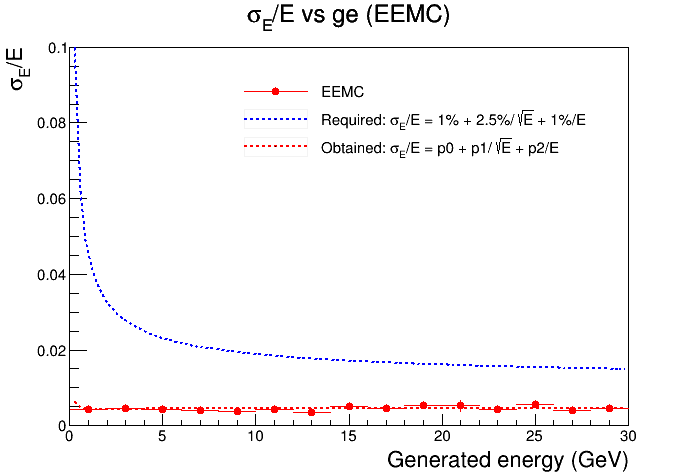
\includegraphics[width=0.5\linewidth]{group1/Resolution_EEMC.png}
		\caption{Energy resolution for electrons shot towards the electron-going electromagnetic calorimeter (EEMC)}
		\label{fig:g1_ch5_img1}
\end{figure}

\textbf{CEMC:}\\
The electrons show a reasonable energy resolution when shot towards barrel electromagnetic calorimeter CEMC. Figure \ref{fig:g1_ch5_img2} shows the energy resolution trend and the parameterized equation for this calorimeter is as follows:
$$\sigma _E/E = 2.05\% + 10.53\%/\sqrt{E} + 2\%/E $$
\begin{figure}
        \centering  
		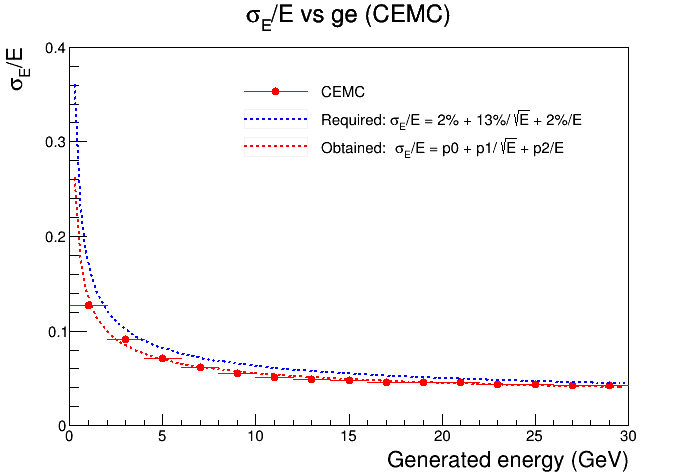
\includegraphics[width=0.5\linewidth]{group1/Resolution_CEMC.png}
		\caption{Energy resolution for electrons shot towards the barrel electromagnetic calorimeter (CEMC)}
		\label{fig:g1_ch5_img2}
\end{figure}
\textbf{FEMC:}\\
The electrons show a good energy resolution when shot towards hadron-going electromagnetic calorimeter FEMC. Figure \ref{fig:g1_ch5_img3} shows the energy resolution trend and the parameterized equation for this calorimeter is as follows:

$$\sigma _E/E = 1.16\% + 4.85\%/\sqrt{E} + 1.08\%/E $$

\begin{figure}
        \centering  
		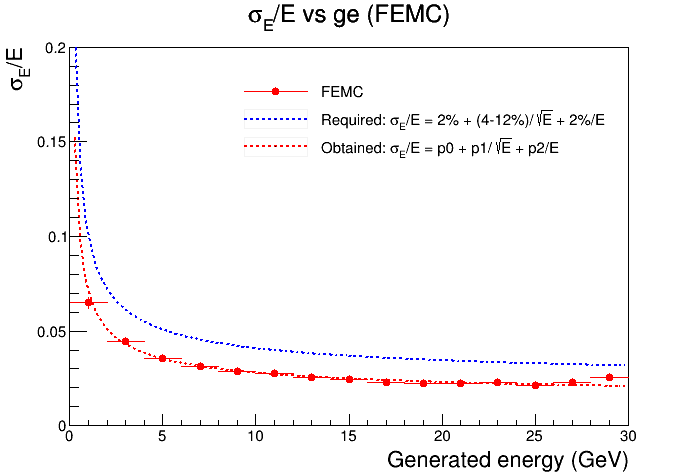
\includegraphics[width=0.5\linewidth]{group1/Resolution_FEMC.png}
		\caption{Energy resolution for electrons shot towards the forward electromagnetic calorimeter (FEMC)}
		\label{fig:g1_ch5_img3}
\end{figure}

\subsection{Pions}
For studying the energy deposition of pions within calorimeters, a large number of pions with following parameters were fired one at a time towards the Fun4All 
calorimeters and the energy response of   calorimeters particularly in barrel and forward region was recorded. In each of these region, the corresponding calorimeters' energy deposition was added up by matching the pseudorapidity covered by the calorimeters. \\
\\
\textbf{Simulations Parameters:}\\
Particle simulated = pi-\\
Total number of events simulated = 100000\\
Generated energies = 0 to 30 GeV \\
Generated pseudo rapidity = -4 to 4\\
Generated polar angle = -pi to pi\\
\\
In order to filter the energies deposited in the various calorimeters in barrel and forward region, following cuts were applied.\\
\\
\textbf{Cuts Applied:}\\
On the individual energies recorded in each tower: MIP theta-dependent energy cut on the electromagnetic calorimeters \\
On the total energy deposited by a single particle in a calorimeter: 100 MeV energy cut\\
\\
The energy resolution obtained for the barrel and forward calorimeters is illustrated below.\\
\\
\textbf{Energy Calibration:}\\
For centering the energy distribution about zero, the following technique was used for electrons:\\
1. Plot the means of the gaussian fits of the various slices of (te-ge)/ge distribution of summed up energies of barrel and forward calorimeters i.e. te (CEMC+HCALIN+HCALOUT), te(FEMC+FHCAL)\\
2. Fit the points with a suitable function (like polynomial)\\
3. Use the obtained fit function to calibrate the original tower energies of each calorimeter by using following formula.\\
$$ te(calibrated) = \frac{te(raw)}{Fit function, f(ge)} $$
\\
The energy resolution obtained for the barrel and forward  calorimeters is illustrated below.\\
\\
\textbf{Barrel Region:}\\
In the barrel region, upon adding the energies recorded in CEMC, HCALIN and HCALOUT, the energy resolution obtained is exhibited in figure \ref{fig:g1_ch5_img4}. At all the energies, the resolution behavior is better than the expected behavior.
\begin{figure}[H]
        \centering  
		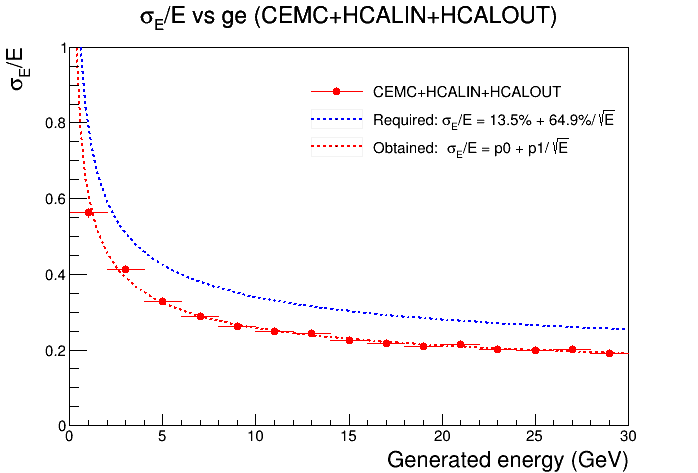
\includegraphics[width=0.5\linewidth]{group1/Resolution_CEMC_HCALIN_HCALOUT.png}
		\caption{Energy resolution for electrons shot towards the forward electromagnetic calorimeter (FEMC)}
		\label{fig:g1_ch5_img4}
\end{figure}
\textbf{Forward Region:}\\
In the forward region, upon adding the energies recorded in FEMC and FHCAL, the energy resolution obtained is exhibited in figure \ref{fig:g1_ch5_img5}. At low energies, the resolution overlaps with expected trend and consistently improves upon increase in generated energies.
\begin{figure}[H]
        \centering  
		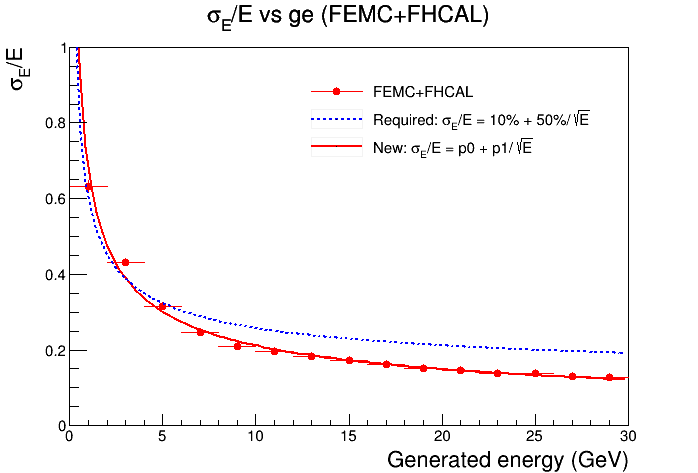
\includegraphics[width=0.5\linewidth]{group1/Resolution_FEMC_FHCAL.png}
		\caption{Energy resolution for pions shot towards the forward calorimeters (FEMC+FHCAL)}
		\label{fig:g1_ch5_img5}
\end{figure}
\textit{It is worth mentioning here that in order to obtain acceptable energy behavior from FEMC, the total event energies recorded in FEMC needed to be multiplied by a factor of 2. This change is illustrated in figure \ref{fig:g1_ch5_img6} and \ref{fig:g1_ch5_img7} compare the original FEMC energy response and the change upon multiplication by a factor of 2 respectively.  }
\begin{figure}[H]
        \centering  
		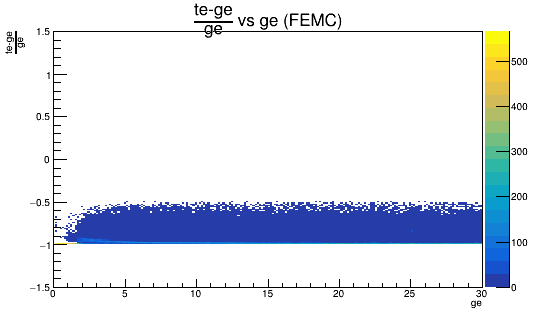
\includegraphics[width=0.5\linewidth]{group1/FEMC.png}
		
		\caption{Energy response of FEMC to pions}
		\label{fig:g1_ch5_img6}
\end{figure}

\begin{figure}[H]
        \centering  
		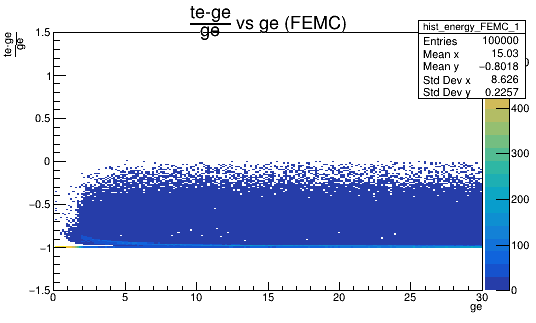
\includegraphics[width=0.5\linewidth]{group1/FEMCx2.png}
		\caption{Energy response of FEMC to pions multiplied by a factor of 2}
		\label{fig:g1_ch5_img7}
\end{figure}


\section{Group 2: Results}
\subsection{Electrons}
\subsection{Simulations Parameters}
\subsection{Implementation and Cuts Applied}
\subsection{Results}


\subsection{Pions}
\subsubsection{Simulations Parameters}
\subsubsection{Implementation and Cuts Applied}
\subsubsection{Results}


